%\documentclass[a4paper,12pt]{exam}

\input{entete_TD}
\begin{document}


\textbf{\large{Écoulement visqueux sur un plan incliné}}


\begin{minipage}{0.7\linewidth}

Et si j'écris moi même des trucs ? Ca marché ou pà ?


On s’intéresse dans cet exercice à l’écoulement d’un film de fluide
visqueux, de viscosité dynamique $\eta$ et de masse volumique $\rho$,
le long d’un plan incliné faisant un angle $\alpha$ avec l’horizontale.

L’écoulement est supposé incompressible.
On se place en régime stationnaire, et on note $h$ l’épaisseur du film
de fluide. Enfin, on suppose que la vitesse du fluide dans ce cas
est de la forme $\vec{v}(M)=v(x,z)\vec{e}_{x}$, avec $x$ l’axe le long
du plan incliné, et que le champ de pression dans le fluide est
$p(x,z)$. L’air extérieur est à la pression $P_0$.

Dans cette situation, on montre que toutes
les forces volumiques s’exerçant sur le fluide doivent se compenser 
exactement.
\end{minipage}
\begin{minipage}{0.3\linewidth}
\begin{center}
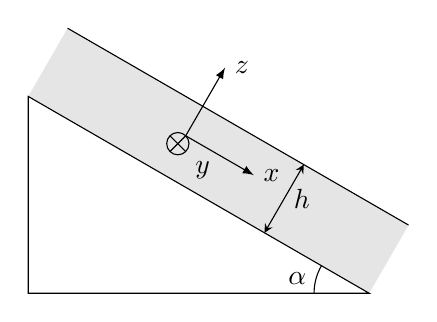
\begin{tikzpicture}
\fill[gray!20] (0,{5*sin(30}) -- ({sin(30)},{5*sin(30)+cos(30)})  -- 
({5*cos(30)+sin(30)},{cos(30)}) -- ({5*cos(30)},0) -- cycle;
\draw (0,0) -- (0,{5*sin(30}) -- ({5*cos(30)},0) -- cycle;
\draw ({5*cos(30)-0.7},0) arc(180:150:0.7) node[midway,left] {$\alpha$};
\draw ({sin(30)},{5*sin(30)+cos(30)}) 
	-- ({5*cos(30)+sin(30)},{cos(30)});
\draw[stealth-stealth] 
(3,{(5*cos(30)-3)*tan(30)}) -- ++ ({sin(30)},{cos(30)}) node[midway,right] {$h$};
\draw[-latex] (2,2) -- ++ ({cos(30)},{-sin(30)}) node[right] {$x$};
\draw[-latex] (2,2) -- ++ ({sin(30)},{cos(30)}) node[right] {$z$};
\draw (2,2) -- (1.8,1.8);
\draw (1.8,2) -- (2,1.8) node[below right] {$y$};
\draw (1.9,1.9) circle ({0.1*sqrt(2)});
\end{tikzpicture}
\end{center}
\end{minipage}


\begin{enumerate}
\item Montrer que la vitesse ne dépend en réalité que de $z$.
	
\item Donner la forme des forces s’appliquant sur le fluide.
	
\item À partir de la condition d’équilibre des forces et des
conditions aux limites, déterminer le champ de vitesse et le champ
de pression en tout point du fluide étudié.
(Les conditions aux limites ici sont données par la pression en $z=h$,
la vitesse en $z=0$ et la contrainte tangentielle en $z=h$, qui peuvent
toutes être exprimées simplement.)
	
\item Calculer le débit massique de l’écoulement sur une largeur
$L$.
	
\end{enumerate}

\end{document}